\section{Distribution of $\lambda$ under additive noise}\label{AdditiveStationary}
\subsection*{Distribution of Additive noise $X \sim \mathrm{Uniform}[0,1]$, $Z \sim \mathcal{N}(0,\sigma^2)$}
\subsubsection{Notations}
\begin{align*}
    x => Current\ position \ of\ \lambda\\
    y => Next\ value\ of\ \lambda\\
    z = y-x \sim \mathcal{N}(0,\sigma^2)\\
    p(y\mid x) => Conditional\ probability\ of\ y\\
    p(y) => probability\ of\ y\\
    p_n(x) = \frac{1}{\sqrt{2\pi}\sigma}\exp^{\frac{-x^2}{2\sigma^2}}\\
    F_n(x_0) = p_n(x < x_0) = \int_{-\infty}^{x_0}p_n(x)dx
\end{align*}
%---------------------------------------------------------
\subsubsection*{Conditional distribution and continuous density}

For $y - x = z \sim \mathcal{N}(0,\sigma^2)$:
\begin{align*}
p(y \mid x) &= p_n(y - x)\big|_{0 < y < 1}
\end{align*}

\textbf{Point masses:}
\begin{align*}
p(y \mid x) &= p_n(k \leq -x)\big|_{y=0} \\
             &= p_n(k \geq 1 - x)\big|_{y=1}
\end{align*}

\textbf{Marginal density for $0 < y < 1$:}
% \begin{align*}
% p(y) &= p_n(y - x)\big|_{0 < y < 1} \\
%      &= F_n(-x)\big|_{y \leq 0} \\
%      &= 1 - F_n(1-x)\big|_{y \geq 1}
% \end{align*}

\begin{align*}
p(y)\big|_{0 < y < 1}
  &= \int_0^1 p(y \mid x)\,dx
   = \int_0^1 p_n(y-x)\,dx \\
  &= -\int_0^1 p_n(y-x)\,d(y-x) \\
  &= -\bigl[F_n(y-x)\bigr]_0^1 \\
\end{align*}

Hence: 
\begin{equation}
    p(y)\big|_{0 < y < 1} = F_n(y) - F_n(y-1)
\end{equation}
%---------------------------------------------------------
\subsubsection*{Point masses via integration by parts}

% \textbf{Aside:} The normal pdf and its CDF satisfy
% \[
%   \frac{1}{\sqrt{2\pi}\,\sigma}\,e^{-x^2/(2\sigma^2)}, \qquad
%   \frac{1}{\sqrt{2\pi}\,\sigma}, \qquad
%   p_n(0)\,e^{-1/(2\sigma^2)}
% \]

\textbf{Mass at $y = 0$:}
\begin{align*}
p(y=0)\big|_{y=0}
  &= \int_0^1 F_n(-x)\,dx
\end{align*}

\textbf{Mass at $y = 1$:}
\begin{align*}
p(y=1)\big|_{y=1}
  &= \int_0^1 \bigl(1 - F_n(1-x)\bigr)\,dx
\end{align*}

\textbf{Substitution} $u = 1-x$, $du = -dx$:
\begin{align*}
  &= -\int_1^0 \bigl(1 - F_n(u)\bigr)\,du
   = -\int_1^0 F_n(-u)\,du
   = \int_0^1 F_n(-u)\,du \\
  &= p(y=0)\big|_{y=1} \quad \Rightarrow \quad p(y=0) = p(y=1)
\end{align*}

\textbf{IBP:} $\int u\,dv = uv - \int v\,du$, with
$u = F_n(-x)$, $v = x$:
\[
  dv = dx, \qquad du = -p_n(-x)\,dx = -p_n(x)\,dx
\]

\textbf{Gaussian identity:}
\[
  x\,p_n(x) = -\sigma^2\,p_n'(x)
  \;\Longrightarrow\;
  x\,p_n(-x)\,dx = -\sigma^2\,d\,p_n(-x)
  \;\Longrightarrow\;
  x\,p_n(n)\,dx = -d\,p_n(\cdot)
\]

\begin{align*}
\int_0^1 F_n(-x)\,dx
  &= \bigl[x\,F_n(-x)\bigr]_0^1 + \int_0^1 x\,p_n(-x)\,dx \\
  &= F_n(-1) + \bigl[p_n(0) - p_n(1)\bigr] \cdot \sigma^2
\end{align*}

Hence:
\begin{equation}
    % \begin{align*}
    p(y=0) = p(y=1) = F_n(-1) + \sigma^2\bigl[p_n(0) - p_n(1)\bigr]
    % \end{align*}
\end{equation}


%---------------------------------------------------------
\subsubsection*{CDF for $0 \leq y_0 \leq 1$}

% \textbf{Summary so far:}
% \[
% \boxed{
% \begin{aligned}
% P(0) = P(1) &= F_n(-1) + \sigma^2\bigl[p_n(0) - p_n(1)\bigr] \\
% p(y)\big|_{0<y<1} &= F_n(y) - F_n(y-1)
% \end{aligned}
% }
% \]

Note: $F_n(x_0) = P_n(x \leq x_0)$.

\textbf{CDF:}
\begin{align*}
p(y < y_0)\\
  &= p(y = 0) + p(0 < y < y_0)\\
  &= F_n(-1) + \sigma^2\bigl[p_n(0) - p_n(1)\bigr]
   + \int_0^{y_0}\bigl(F_n(y) - F_n(y-1)\bigr)\,dy
\end{align*}

\textbf{Antiderivative of $F_n$} (IBP):
\begin{align*}
\int F_n(y)\,dy
  &= F_n(y)\cdot y - \int y\,p_n(y)\,dy \\
  &= F_n(y)\,y + \sigma^2\,p_n(y) + C
\end{align*}

\textbf{Definite integral:}
\begin{align*}
\int_0^{y_0} F_n(y)\,dy
  &= y_0\,F_n(y_0) + \sigma^2\bigl[p_n(y_0) - p_n(0)\bigr]
\end{align*}

\textbf{Shifted integral} via $u = y-1$, $du = dy$, $y=0 \Rightarrow u=-1$, $y=y_0 \Rightarrow u=y_0-1$:
\begin{align*}
\int_0^{y_0} F_n(y-1)\,dy
  &= \int_{-1}^{y_0-1} F_n(u)\,du
   = \int_{-1}^{0} F_n(u)\,du + \int_0^{y_0} F_n(u)\,du
\end{align*}

Therefore:
\begin{align}
p(y < y_0) &= p(0)
   - \int_{-1}^{y_0-1} F_n(y)\,dy
   + \int_0^{y_0} F_n(y)\,dy
\end{align}

%---------------------------------------------------------
\subsubsection*{Evaluating the CDF explicitly}

\[
\int F_n(y)\,dy = y\,F_n(y) + \sigma^2\,p_n(y) + C
\]

\begin{align*}
p(y \leq y_0)
  &= p(0)
   - \int_{-1}^{y_0-1} F_n(y)\,dy
   + \int_0^{y_0} F_n(y)\,dy \\[6pt]
  &= p(0)
   - \bigl[(y_0-1)\,F_n(y_0-1) - \sigma^2\,p_n(y_0-1)\bigr] \\
  &\quad - \bigl[(-1)\,F_n(-1) + \sigma^2\,p_n(-1)\bigr] \\
  &\quad + y_0\,F_n(y_0) + \sigma^2\,p_n(y_0) - \sigma^2\,p_n(0) \\[6pt]
  &= F_n(-1) + \sigma^2\bigl[p_n(0) - p_n(1)\bigr] \\
  &\quad - (y_0-1)\,F_n(y_0-1) - \sigma^2\,p_n(y_0-1) \\
  &\quad - F_n(-1) + \sigma^2\,p_n(-1) \\
  &\quad + y_0\,F_n(y_0) + \sigma^2\,p_n(y_0) - \sigma^2\,p_n(0) \\[6pt]
  &= y_0\,F_n(y_0) - (y_0-1)\,F_n(y_0-1)
   + \sigma^2\bigl[p_n(y_0) - p_n(y_0-1)\bigr] \\[6pt]
  &= y_0\,F_n(y_0) + (1-y_0)\bigl(1 - F_n(1-y_0)\bigr)
   + \sigma^2\bigl[p_n(y_0) - p_n(1-y_0)\bigr]
\end{align*}

%---------------------------------------------------------
\subsubsection*{Final form and complement}

\[
p(y \leq y_0)
  = y_0\,F_n(y_0)
  + (1-y_0)\bigl(1 - F_n(1-y_0)\bigr)
  + \sigma^2\bigl[p_n(y_0) - p_n(1-y_0)\bigr]
\]

\textbf{Complement $P(y_0 \leq Y \leq 1)$:}
\begin{align*}
p(y_0 \leq Y \leq 1)
  &= 1 - p(Y < y_0) \\
  &= 1 - \Bigl[
      y_0\,F_n(y_0)
      + (1-y_0)\bigl(1-F_n(1-y_0)\bigr)
      + \sigma^2\bigl[p_n(y_0) - p_n(1-y_0)\bigr]
    \Bigr]
\end{align*}

\textbf{Substitution} $y_0 = 1 - y'$:
\begin{align*}
  &= 1 - \Bigl[
      (1-y')\,F_n(1-y')
      + y'\bigl(1 - F_n(y')\bigr)
      + \sigma^2\bigl[p_n(1-y') - p_n(y')\bigr]
    \Bigr] \\[4pt]
  &= 1 - (1-y')\,F_n(1-y') - y' + y'\,F_n(y') \\
  &\quad - \sigma^2\,p_n(1-y') + \sigma^2\,p_n(y') \\[4pt]
  &= (1-y')\bigl(1 - F_n(1-y')\bigr)
   + y'\,F_n(y')
   + \sigma^2\bigl[p_n(y') - p_n(1-y')\bigr]
\end{align*}

%---------------------------------------------------------
\subsubsection*{Summary and numerical example}

\[
\boxed{
\begin{aligned}
p(0) = p(1)
  &= F_n(-1) + \sigma^2\bigl[p_n(0) - p_n(1)\bigr] \\
p(y)\big|_{0<y<1}
  &= F_n(y) - F_n(y-1)
\end{aligned}
}
\]

\begin{equation}
p(y \leq y_0)
  = y_0\,F_n(y_0)
  + (1-y_0)\bigl(1 - F_n(1-y_0)\bigr)
  + \sigma^2\bigl[p_n(y_0) - p_n(1-y_0)\bigr]
  \label{additiveCDF}
\end{equation}

\textbf{Note:} this also equals $p(y_0 \leq Y \leq 1)$ by symmetry. \\[6pt]

% We find a reasonable strong agreement between the simuated and analytically derived distributions, as shown below. 

% \begin{figure}
%     \centering
%     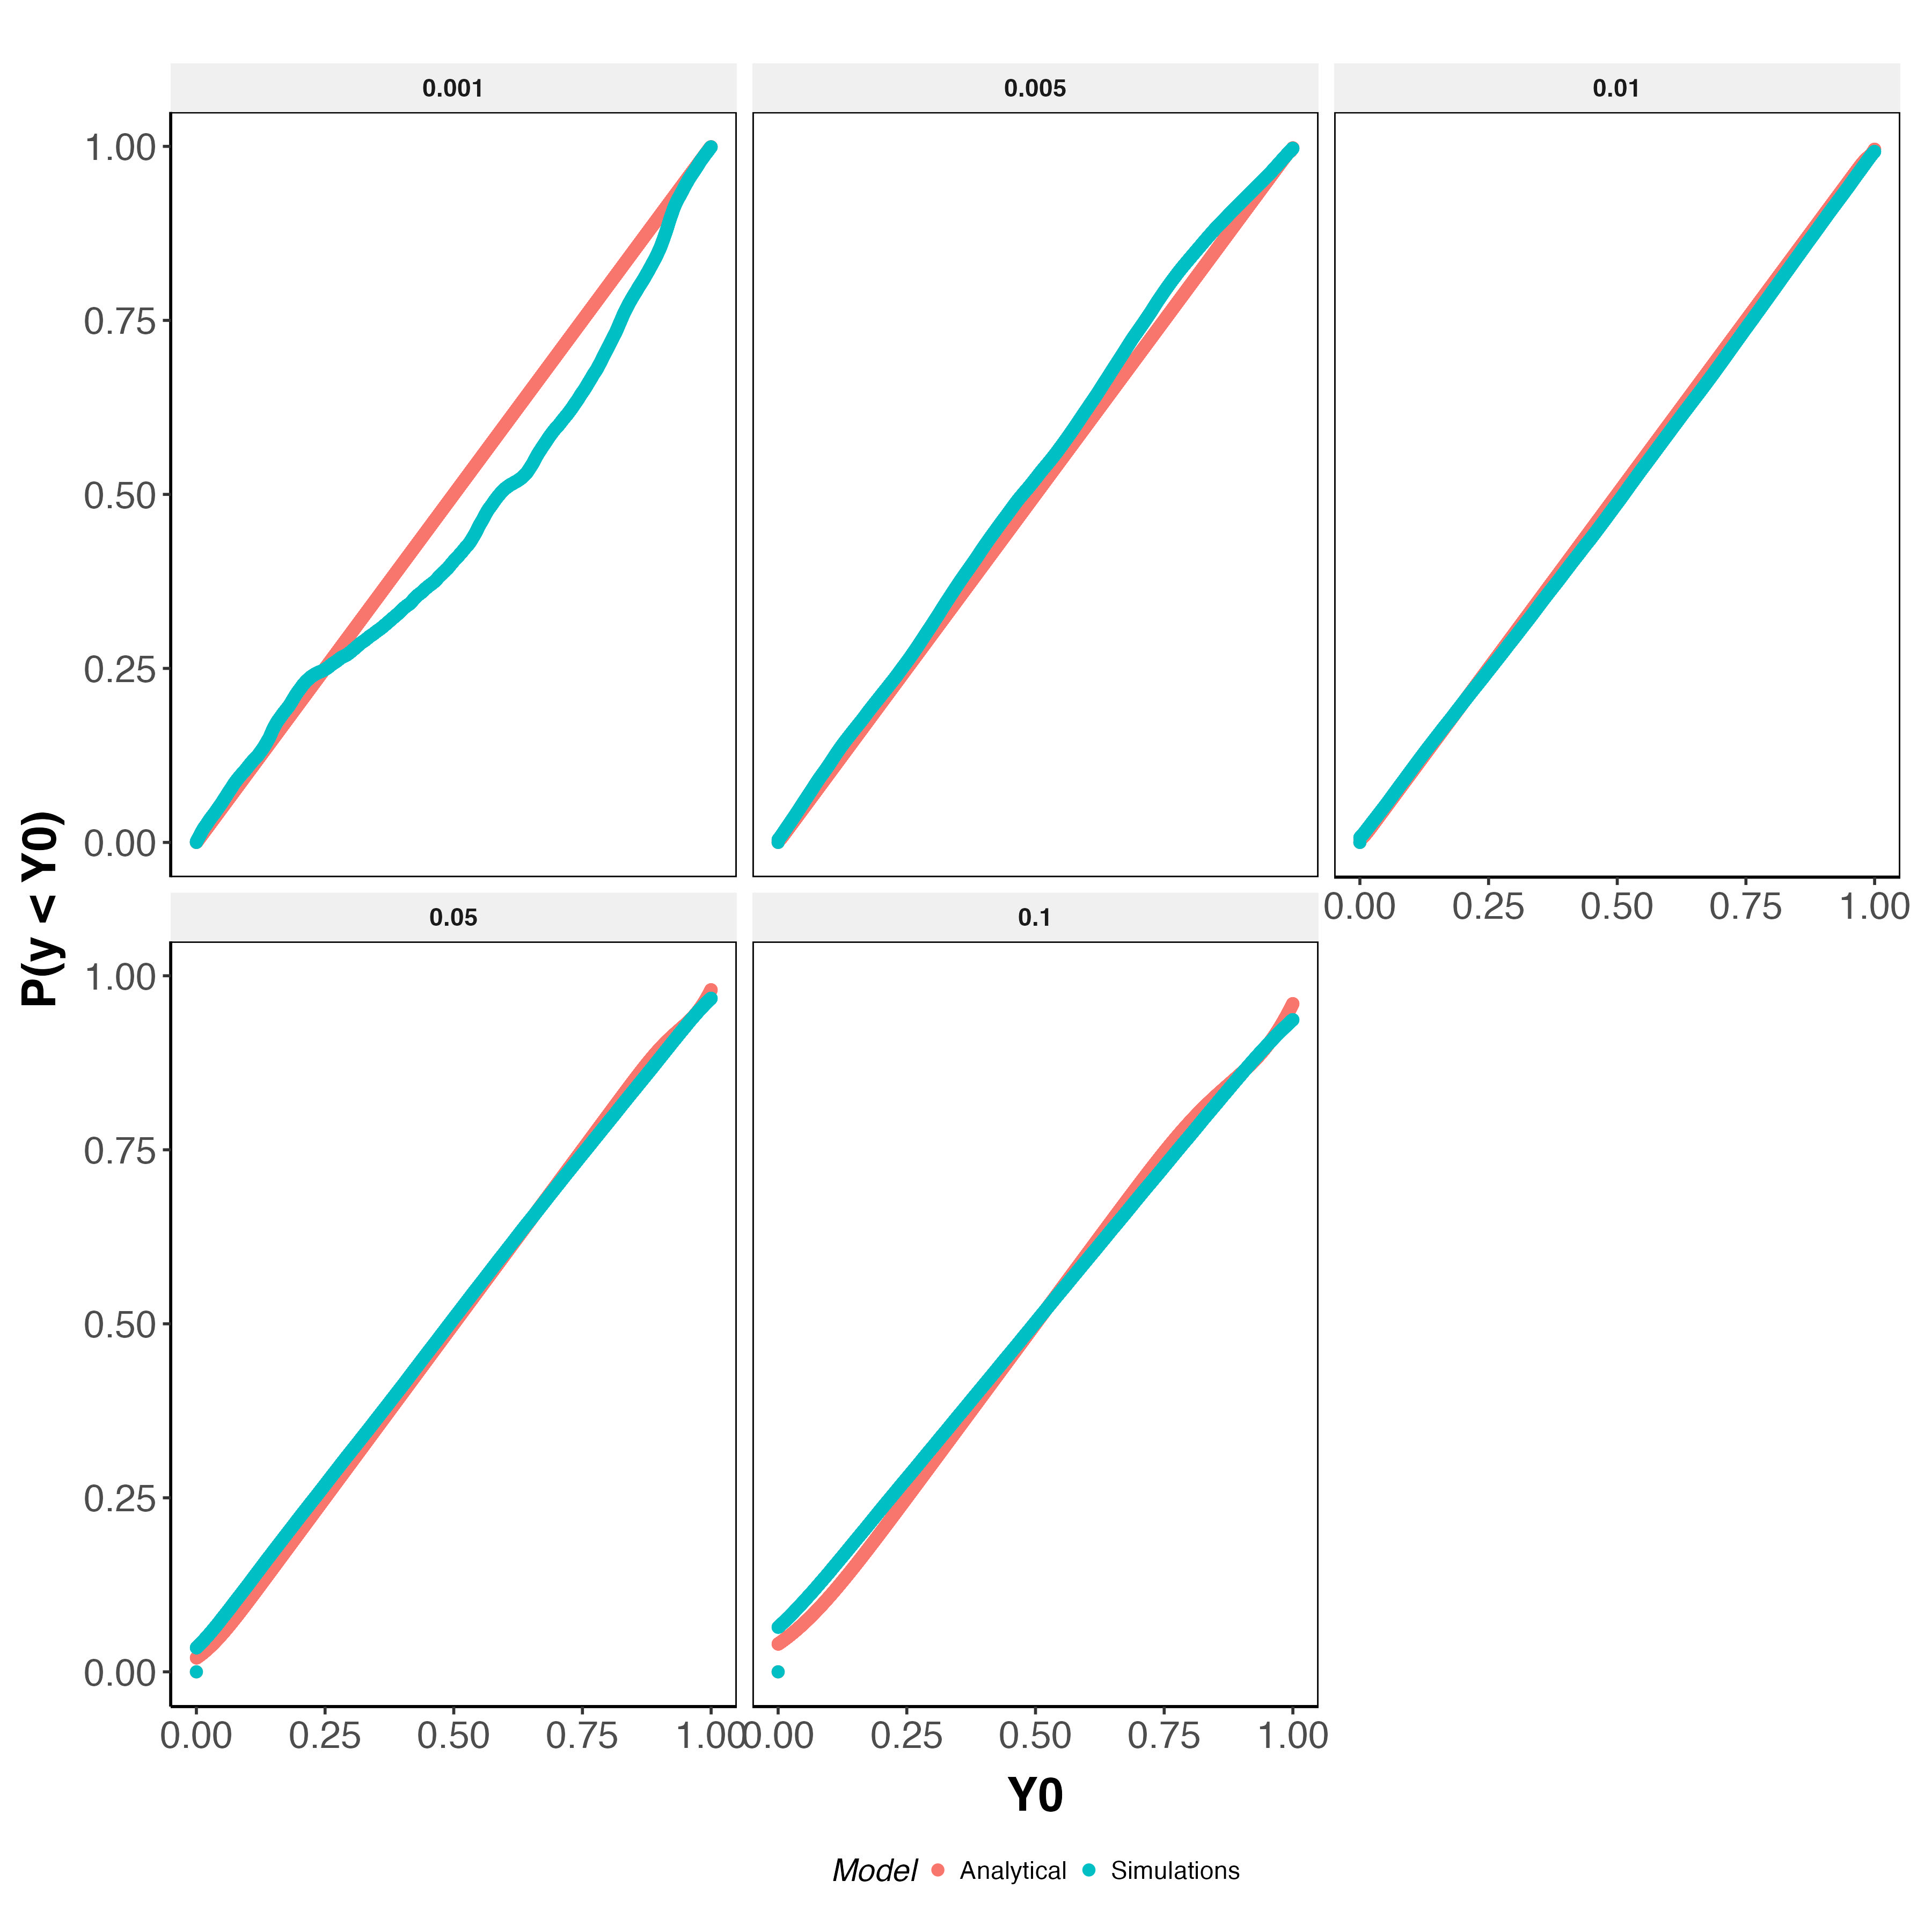
\includegraphics[width=\linewidth]{AditiveNoiseFigures/prob_dist_compare.jpg}
%     \caption{\textbf{Comparision of CDFs generated from simulations and the analytical calculations} Each panel shows the cumulative distribution obtained from Eq \ref{additiveCDF} (red) and numerically calculated trajectories (green). The CDFs agree well with each other, with minor differences that should not have any strong impact on sampling lambda values.} 
%     \label{fig:noiseDist}
% \end{figure}

